\documentclass[UTF8,10pt,a4paper]{ctexart}

\usepackage[top=1in, bottom=1in, left=1in, right=1in]{geometry}
\usepackage{indentfirst}
\usepackage{setspace}
\usepackage{color}

%font
\usepackage{fontspec,xltxtra,xunicode}
\setromanfont{STZhongsong}

%section
\ctexset{section/format=\Large\bfseries}


%table
\usepackage{multicol}
\usepackage{multirow}
\usepackage{booktabs} %toprule...
\usepackage{arydshln} %虚线
\usepackage{dashrule} %虚线

%list


%figs
\usepackage{graphicx}
\usepackage{subfigure}
\usepackage{float}
\graphicspath{{./figs/}{./}{./figs2/}}

%logo
\usepackage{fancyhdr}
\pagestyle{fancy}
\lhead{\includegraphics[scale=0.1]{BGIlogo.png}}  %在此处插入logo.pdf图片

%附录
\usepackage[titletoc]{appendix}

%超链接
%\usepackage[hyperfootnotes=true]{hyperref}
\usepackage[colorlinks,
            linkcolor=red,
            anchorcolor=blue,
            citecolor=green,
            urlcolor=blue]{hyperref}

%原文照列
\usepackage{verbatim}
\usepackage{clrscode}
\usepackage{listings} %插入代码

\lstset{numbers=left, %设置行号位置
        backgroundcolor=\color[RGB]{245,245,244},
        basicstyle=\footnotesize,
        showstringspaces=false,
        numberstyle=\tiny, %设置行号大小
        keywordstyle=\color{blue}, %设置关键字颜色
        commentstyle=\color[cmyk]{1,0,1,0}, %设置注释颜色
        frame=single, %设置边框格式
   %     escapeinside=``, %逃逸字符(1左面的键),用于显示中文
       basicstyle=\scriptsize\ttfamily,
        breaklines, %自动折行
        extendedchars=false, %解决代码跨页时,章节标题,页眉等汉字不显示的问题
        xleftmargin=2em,xrightmargin=2em, aboveskip=1em, %设置边距
        tabsize=4, %设置tab空格数
        showspaces=false, %不显示空格
        %belowcaptionskip=1\baselineskip,
        stringstyle=\color{orange}
        }

\title{GaeaAnnotator说明文档{\small (v0.1)}}
\author{\href{http://bigdata.genomics.cn/}{大数据计算组} \and
\href{mailto:huangzhibo@genomics.cn}{黄志博}}
\date{\today}

%\author{\textcolor{blue}{huangzhibo@genomics.cn}

\begin{document}
\maketitle
\vspace{3em}
%\tableofcontents
\tableofcontents\thispagestyle{empty}
\newpage
\setlength{\parskip}{1ex plus 0.5ex minus 0.2ex}


%\setcounter{subsection}{0}

\section{概述}
\subsection{开发目的}
随着高通量测序技术的发展及其越来越广泛的应用,当今世界正在累积巨量的NGS数据,而对NGS变异数据的注释和解读已经成为快速理解这些测序数据的一个瓶颈。为了实现对大量变异数据的快速注释,我们决定基于hadoop平台开发并行化的注释程序。

\subsection{开发人员}
\begin{multicols}{5}
\begin{itemize}
\item \href{mailto:huangzhibo@genomics.cn} {黄志博 }
\item  \href{mailto:zhangyong2@genomics.cn}{张勇}
\item \href{mailto:lishengkang@genomics.cn}{李胜康}
\item \href{mailto:shiquan@genomics.cn}{石泉}
\item 肖鹏
\end{itemize}
\end{multicols}

\section{程序特性说明}
\subsection{reference版本}
目前暂只支持hg19/GRCh37版本,后续会导入GRCh38版本数据库。
\begin{itemize}
	\item hg19/GRCh37
        \item[$\circ$] GRCh38
\end{itemize}

\subsection{注释变异类型}
\begin{figure}[htbp]
\begin{center}
\label{variantType}
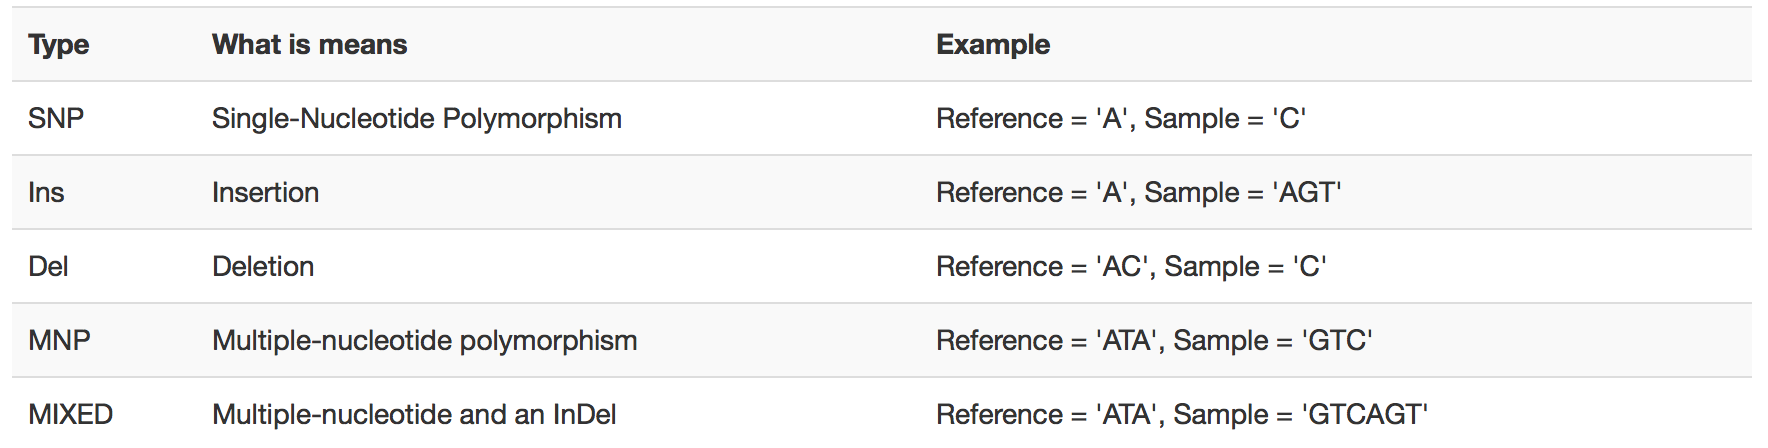
\includegraphics[width=15cm]{variantType.png}
%\caption{要注释的变异类型}
\end{center}
\end{figure}

\subsection{输入输出格式}
\begin{itemize}
\item 输入文件: VCF 
\item 输出文件: TSV, Excel\footnote{使用工具/ifs4/ISDC\_BD/GaeaProject/software/GaeaAnnotator/toExcel.sh将TSV格式结果转换成Excel,注意TSV文件不能过大}
\end{itemize}

\subsection{运行环境及开发语言}
\begin{itemize}
\item 运行环境: Hadoop 2.6.0 + Hbase 1.2.0
\item 开发语言: Java
\end{itemize}

\subsection{性能}
\begin{itemize}
\item 在BGI hadoop50集群注释单个WGS变异数据(NA2878样本4987513条变异数据)用时约11分钟。
\end{itemize}

\section{注释数据库}
对NGS变异信息进行Gene注释、功能预测和致病性预测等。

\subsection{基因及转录本信息数据库}
\begin{itemize}
	\item UCSC refgene
        \item ENSEMBL Gene
        \item[$\circ$] UCSC Known Gene
         \item[$\circ$] CCDS
\end{itemize}

\subsection{其他可用数据库}
详细信息见\href{https://github.com/huangzhibo/Documents/blob/master/GaeaAnnotator/AnnotationDatabase.md}{AnnotationDatabase.md}, \\
\indent 注释条目列表见/ifs4/ISDC \_BD/huangzhibo/Data/database/header/。

\begin{itemize}
\item ESP6500
\item G1000
\item EXAC
\item dbSNP
\item HGNC
\item gwasCatalog
\item CLINVAR
\item dbNSFP
\item HGMD
\end{itemize}


\section{使用说明}
\subsection{配置文件}
配置文件中需要指明以下几项内容:
\begin{description}
\item[ ref : ]  reference版本
\item[ GeneInfo : ] 指定基因及转录本信息文件
\item[ GeneInfoType : ] 指定基因及转录本信息数据库版本
\item[ \{dbName\}.fields : ]  根据注释header List中\footnote{见/ifs4/ISDC \_BD/huangzhibo/Data/database/header/}的条目设置各数据库的注释字段。不设置或值为空则视为不对该数据库进行注释。
\end{description}

\begin{description}
\item[ 配置文件示例:]  /ifs4/ISDC\_BD/GaeaProject/software/GaeaAnnotator/config.properties
\end{description}
\lstinputlisting[]{source/config.properties}

\subsection{运行}
\begin{description}
\item[ 执行方式:]  hadoop jar GaeaAnnotator.jar  [options]
\item[ 程序路径:]   /ifs4/ISDC\_BD/GaeaProject/software/GaeaAnnotator/GaeaAnnotator.jar
\item[ 示例脚本:]  /ifs4/ISDC\_BD/GaeaProject/software/GaeaAnnotator/run.sh
\end{description}
目前只开放hadoop50集群作为注释计算平台,使用方法见示例脚本。程序具体参数如下:
\lstinputlisting[]{source/usage.txt}

说明:
\begin{description}
\item[-i ]  须指定非压缩VCF文件。
\item[-o ] 本地输出文件(gz压缩)。
\item[-r ]  vcf对应的reference序列Gaea索引文件,见/ifs4/ISDC\_BD/GaeaProject/reference/
\item[-c ] 配置文件
\item[-m ]  mapper数目,根据集群情况设定。
\end{description}

\subsection{结果展示}
\begin{figure}[htbp]
\begin{center}
\label{variantType}
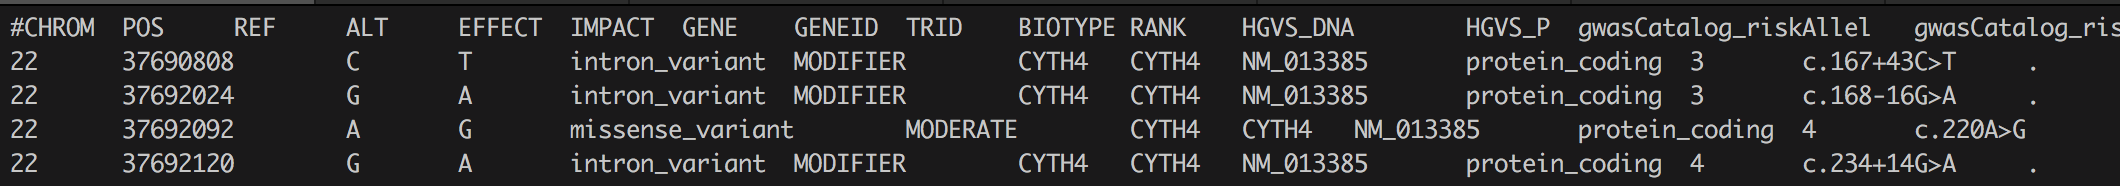
\includegraphics[width=15cm]{annoResultsTsv.png}
\caption{TSV格式注释结果}
\end{center}
\end{figure}

\begin{figure}[htbp]
\begin{center}
\label{variantType}
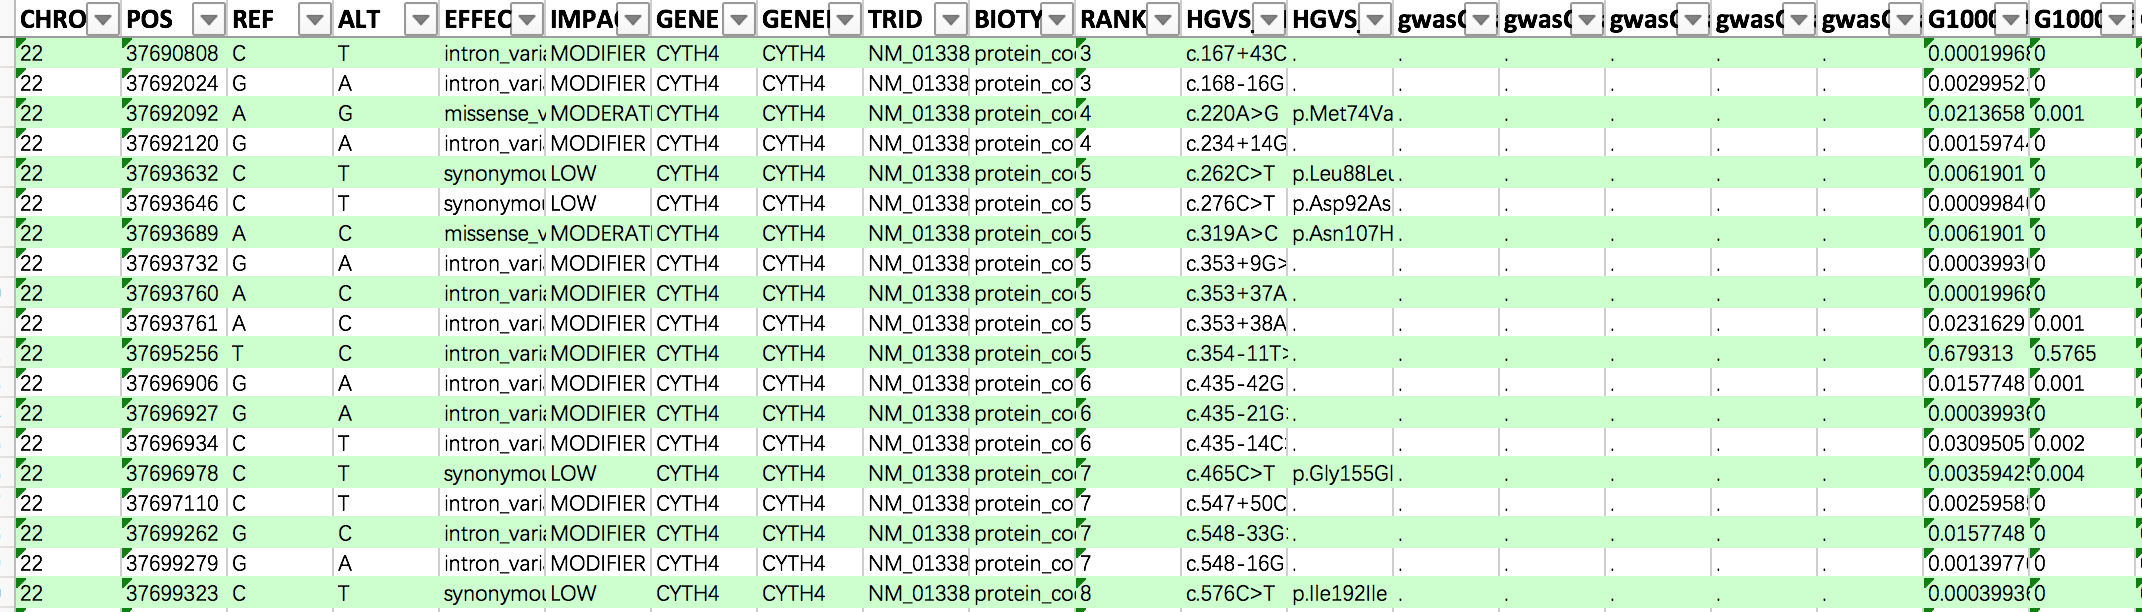
\includegraphics[width=15cm]{annoResults.png}
\caption{Excel格式注释结果}
\end{center}
\end{figure}


\end{document}
